%% paper.tex
%% V1.4b
%% 2017/03/05
%% by HSNL, NTHU


\documentclass[conference]{IEEEtran}

\usepackage{graphicx}
\usepackage{indentfirst}
\usepackage{cite}
\usepackage{url}
\usepackage{hyperref}
\usepackage{amsmath}
\usepackage{enumerate}
\usepackage[flushleft]{threeparttable}
\usepackage[super]{nth}


\begin{document}

\title{Performance Optimization of Service Chain for vCPE in Small Networks with OpenFlow Switch}

\author{
\IEEEauthorblockN{
Nen-Fu Huang\IEEEauthorrefmark{1},
Chi-Hsuan~Li\IEEEauthorrefmark{1},
Chia-Chi~Chen\IEEEauthorrefmark{1}, and
I-Hsien~Hsu\IEEEauthorrefmark{1}}

\IEEEauthorblockA{
\IEEEauthorrefmark{1}
Department of Computer Science National Tsing Hua University, Hsinchu, Taiwan \\
Email: nfhuang@cs.nthu.edu.tw
}
}

% make the title area
\maketitle


\begin{abstract}
% Virtual Customer Premise Equipment (vCPE) is one of the game-changing applications that could reduce OPEX and CAPEX simultaneously. This service is based on a complex software architecture with several technologies behind like Virtualized Network Functions (VNFs) and Service Chaining. Many researches have discussed algorithm or mechanism about linking multiple VNFs as a single Network Function Virtualization (NFV) in order to form a service chain in a virtual environment. Nevertheless, the waste of hardware resource and characteristic of SDN switch has never been mentioned before in this architecture. In this paper, a vCPE framework with multiple flow table management is implemented. This proposed vCPE framework is able to create a SDN-enabled VNF which could be deployed as the edge by employing both resources in SDN switch and on the cloud. Last but not least, the system is also integrated with an application identification engine based on machine learning algorithms thus providing flow control in the vCPE framework with confidence.
\end{abstract}

% Note that keywords are not normally used for peerreview papers.
\begin{IEEEkeywords}
Software defined network, network function virtualization, NFV orchestration, virtual customer premise equipment, OpenFlow, multiple flow tables
\end{IEEEkeywords}

\IEEEpeerreviewmaketitle{}


% Introduction
% First paragraph of paper need be big Alhabet
\section{Introduction}
\section{Related Work}

\section{System Description}
\subsection{Overview of Network Functions} \label{ssec:desc_nfv_overview}
Our network functions (Fig. \ref{fig:desc_nfv_overview}) are designed with SDN-enabled NFV architecture concept \cite{sdn-enabled}, using the synergies between computer infrastructures (NFVs) and network infrastructures (NFVIs) \cite{nfv2014-v121, nfv2015}.
An NFV is a VNF controller, mainly used for addressing stateful processing and NFVI is an SDN switch used for stateless processing.

\begin{figure}[!t]
\centering
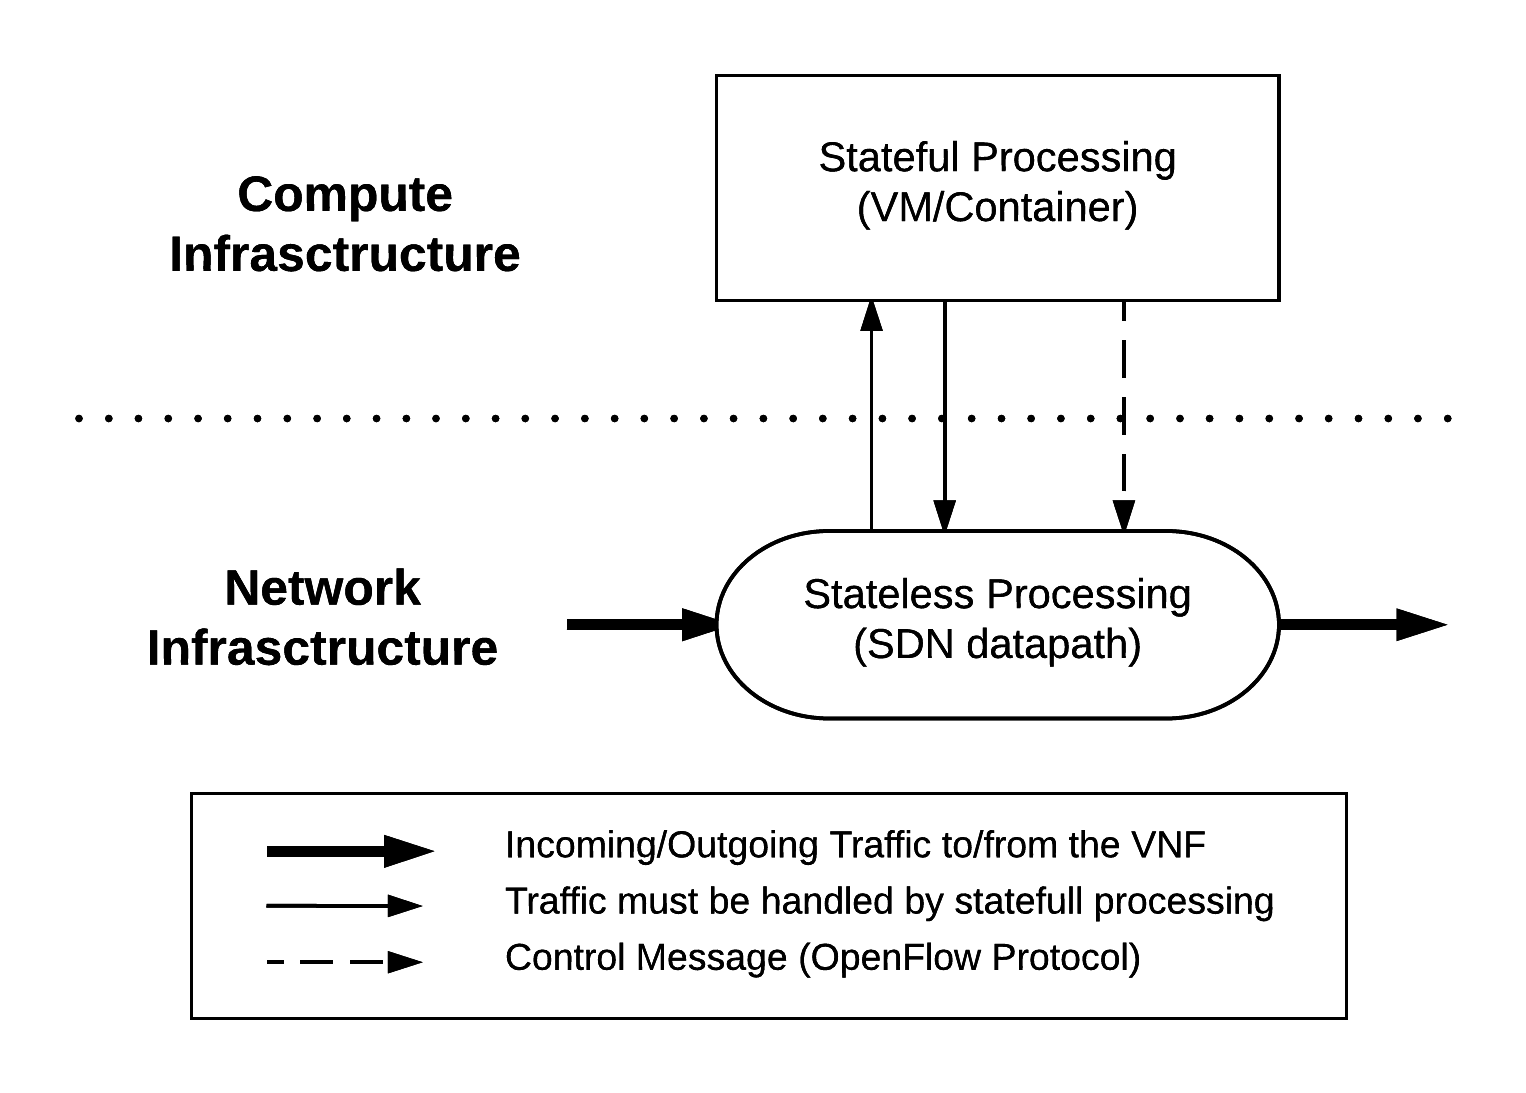
\includegraphics[width=2.5in]{./figures/desc_nfv_overview}
\caption{Overview of network functions.}
\label{fig:desc_nfv_overview}
\end{figure}

\subsubsection{Stateful Processing Component (VNF Controller in VM or Container)}
This component is used to control the workflow, maintain the state associated with the VNF, and provide an interface for service providers or customers to configure and update the behavior of the stateless datapath processing component. We used an SDN controller to implement the VNF controller; and notably, we use southbound APIs of the SDN controller framework to manage the interface between the stateful and stateless components with the OpenFlow protocol, which was originally designed for this purpose.

\subsubsection{Stateless Processing Component (SDN Datapath)}
Stateless processing component is implemented by SDN datapath resources and is optimized for data plane traffic processing. Because an SDN switch can be decoupled with control plane and data plane, the switch can accept the control messages from the stateful processing component.

By using the advantages of this architecture, we can assign stateless or light-weight state work to the SDN switch (e.g., packet filtering and packet counting) to reduce the load on the computing resources. If we want to update our service, we are required to update only the stateful component, because the stateless component merely follows the commands from the stateful component.



\subsection{Service Deployment Model}
Unlike a related study that explored the virtualization of network function in PE devices \cite{vcpe-enhance}, we introduced a network function service deployment model based on the NetFATE (Network Function at the Edge) approach \cite{netfate}; the architecture of the model is presented in Fig. \ref{fig:desc_nfv_overview}. Because computing infrastructures involves algorithms and policies and the generic network devices perform only stateless processing, the customers need to simply purchase a general SDN switch for their home gateway. They can obtain a different network function service by subscribing to a different VNF controller through our vCPE platform.

Fig. \ref{fig:desc_service_deployment} illustrates the service deployment model. Each green area is a local network domain of the customer. An SDN switch is presented at the gateway of this domain. The customer can subscribe to our vCPE service through our dashboard. After subscription, the vCPE system creates a new Docker container or new VM in which an SDN controller is run. The customer only needs to set up the gateway SDN switch to connect the SDN controller through the OpenFlow protocol; thereafter, the switch executes the service.

\begin{figure}[!t]
\centering
\includegraphics[width=3in]{./figures/desc_service_deployment}
\caption{Service deployment model.}
\label{fig:desc_service_deployment}
\end{figure}



\subsection{vCPE System Architecture}
The architecture (Fig. \ref{fig:desc_vcpe_framework}) is adapted from the NFV-MANO architectural framework in \cite{nfv2014-v111}, including an infrastructure controller, an infrastructure orchestrator, a cloud database, VNF controllers and a VNF Orchestrator. Each component is introduced in the following subsection.

\begin{figure}[!t]
\centering
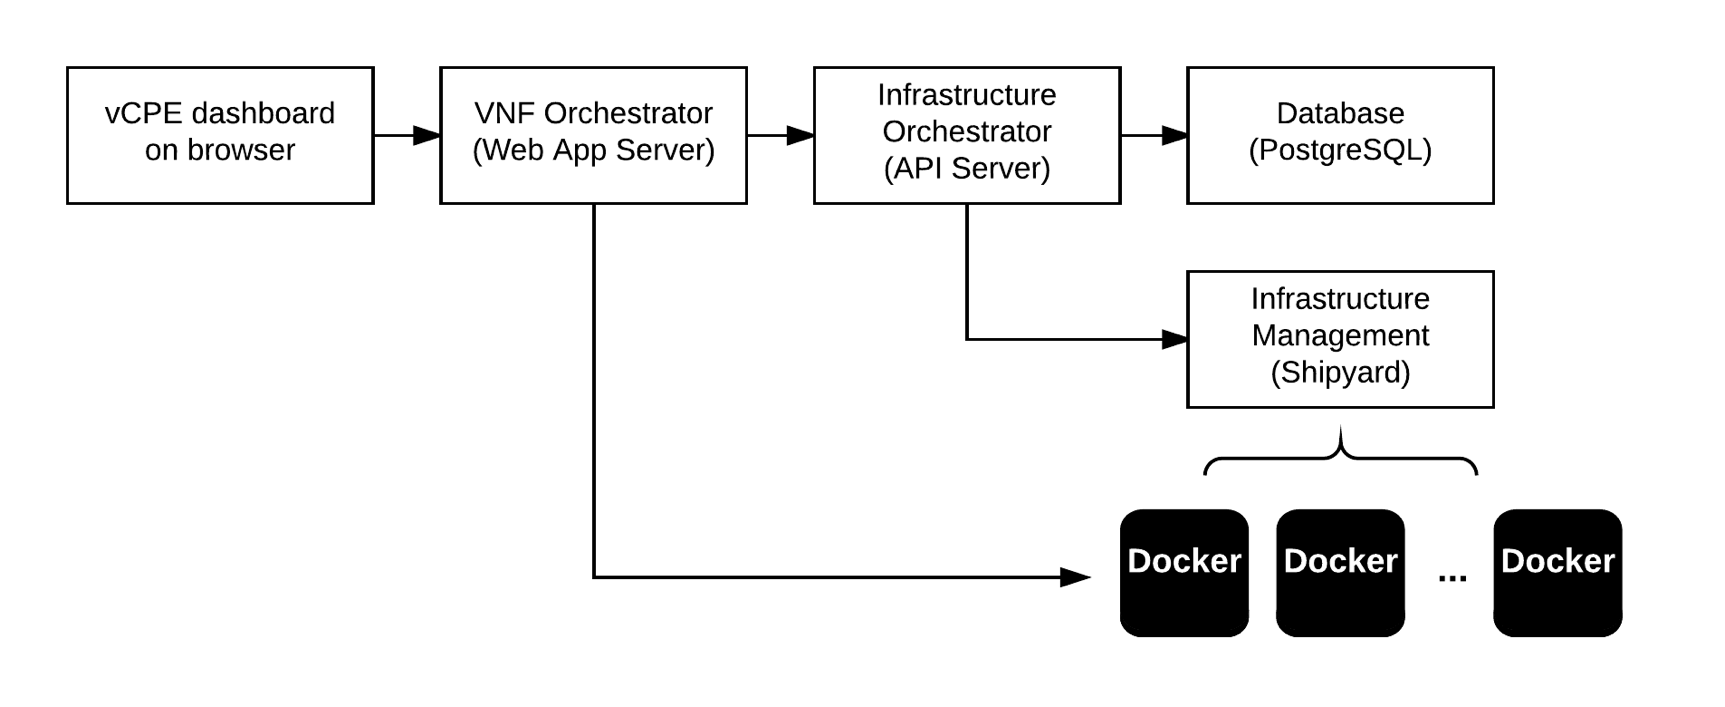
\includegraphics[width=3in]{./figures/desc_vcpe_framework}
\caption{Architecture of the vCPE framework.}
\label{fig:desc_vcpe_framework}
\end{figure}

\subsubsection{Infrastructure Controller}

The infrastructure controller comprises a Docker management server that can manage the Docker resources like containers and images and a OpenStack server that can manage the VM resources. The infrastructure controller does not manage customer authentication or maintaining the state of the running service; however, it follows the request from the infrastructure orchestrator to create, delete, start, stop, and inspect containers and VMs.

\subsubsection{Infrastructure Orchestrator}
The infrastructure orchestrator plays a key role in our system. It connects and automates the workflows when our services are deployed. When a customer subscribes to our service, the infrastructure orchestrator first authenticates the customer, calls the infrastructure controller to create a container or a VM for the customer, and then updates the information in the database. The infrastructure orchestrator controls the entire life-cycle of our vCPE services.

\subsubsection{Cloud Database}
The cloud database is used for restoring the meta data of our vCPE services, which include each customer’s credentials, customer’s container/VM settings, and virtual CPE service states. The cloud database employs PostgreSQL, which is an open source, easily customizable and object-relational database system. Only the infrastructure orchestrator has permissions to access the cloud database.

\subsubsection{VNF Controllers}
VNF controllers comprises an SDN controller developed using Ryu framework \cite{web:ryu} and a remote launcher module. The SDN controller does not have a remote launcher module for remotely executing an SDN controller. We built a light-weight server as a launcher module to resolve this problem. The remote launcher module monitors the SDN controller process ID (PID) and kills the SDN controller PID on demand. Once the infrastructure controller  creates the container or the VM, the remote module will initially runs, waiting for requests from VNF Orchestrator. The details of an SDN controller design are presented at Section \ref{sec:mft}.

\subsubsection{VNF Orchestrator}
The VNF orchestrator is a web application server hosted on Amazon web server, and provides to customers an online dashboard for vCPE services management and configuration. Through the web-based UI provided by the VNF orchestrator, customers can subscribe to the desired service without typing any command through the command line interface. After receiving the subscription message, the VNF orchestrator requests the infrastructure orchestrator to create a new VNF controller, and then sends the virtual CPE configuration to the new VNF controller. Based on configuration demands under different conditions, the network administrator can select any of the listed network functions on the dashboard, such as Firewall, NAT, DHCP, and quality of service (QoS) management.


\section{Network Function With Multiple Flow Table Management Model} \label{sec:mft}

\begin{figure*}[!t]
\centering
\includegraphics[width=6in]{./figures/mft_table_overview}
\caption{Flow table order of vCPE service.}
\label{fig:mft_table_overview}
\end{figure*}

\subsection{Multiple Flow Tables Strategy}
In subsection \ref{ssec:desc_nfv_overview}, we introduce the vCPE service design architecture. The network functions are managed through cooperation between the SDN controller on the cloud and SDN switch at the local network gateway. The controller transforms the network functions into a series of OpenFlow rule requests and sends it to the SDN switch. Following the orders from the controller, the SDN switch inserts the rules into its flow tables, examines the incoming packets against the flow entry match fields, and executes the actions in matching rules. The flow table \cite{sdn-ft} defines all matching and corresponding processing, thus playing an important role in the executive network function.

We found that a single flow table restricts the implementation of our network functions. In \cite{onf-multi-tables}, two conditions under which a single flow table is too restrictive were reported. The first is a condition where a single packet must perform independent actions based on matching with different fields. The second is a condition where the packet requires two-stage processing. To satisfy both conditions, we implemented the network functions by using a multiple flow table strategy.

Before we discuss about the multiple flow table strategy, we introduce the pipeline of OpenFlow flow table first \cite{sp:openflow13}. The processing of each packet always starts at the first flow table. When processed by a flow table, the packet is matched the flow entries of the flow table and adds corresponding action to the instruction set. The packet can executes the instrcution set immediately, or execute after finishing the journey in switch. A flow entry can direct a packet to next table by go-to action. In our multiple flow table management model, we will set the go-to-next-table action as the table-miss action. Therefore, the packet is processed table-by-table in a certain sequence.

In a multiple flow table strategy, it is most important to determine which flow table the rules should be inserted into. We used the network function as a demarcation, that is, SDN applications responsible for specific network functions inserted rules into one specific flow table to enable us to focus on the design of the network function itself. However, the order of the flow table and the sequence of the network functions become crucial. This can be addressed by considering the type of match and action in the rules generated by the network function.

The network functions of vCPE services are the firewall service, NAT, DHCP, forwarding, and QoS. The order of each function was determined as shown in Fig. \ref{fig:mft_table_overview} (note that the flow tables are counted from zero). Each packet In the following sections, we introduce the method of implementing these network functions, the type of rules to be inserted into the SDN switch, and the effect of these rules on deciding the order of the flow tables



\subsection{Service Control}
Service control is used to enable or disable services. To enable a service, the table-miss rule should be modified. A packet-in rule is always placed in the flow table of the last active service as a table miss in case there is no corresponding rule. To enable the service chain, the rules of each service except the last service contain an additional action, ``go to next flow table'', which enables the packets to continue to pass through all active services.

To disable a service, we must not only modify the table-miss rule but also add an enforce rule. Each enforce rule has maximum priority with the action, ``go to next flow table''. It indicates that packets still pass through the disabled service’s table, but ignore other rules and proceed to the next flow table.



\subsection{Firewall}
The firewall service can dynamically block traffic and prevent the packets from causing a packet-in event.

On the dashboard, we can specify the blocking policies. There are 3 kinds of policies:
\begin{itemize}[\IEEEsetlabelwidth{Z}]
\item block any traffic from a source IP or destination IP address;
\item block traffic based on known layer 4 protocols, such as SSH and HTTP;
\item block traffic to customize layer 4 ports of a host.
\end{itemize}

For different policies, the controller applies corresponding rules to the SDN switch. After the policies are set, the blocking rules are immediately installed. Subsequently, any traffic that satisfies the blocking criteria is dropped. Normal traffic is unaffected.

As shown in Table \ref{table:fw}, all the actions of flow entries are dropped. The first rule illustrates that SSH connection with the source IP address 192.168.2.1 is blocked. The second rule indicates that the flow entry blocks the Telnet protocol.

In our multiple flow table model, the firewall service is located in flow table 1 because once packets are detected by the blocking rules, they do not need to be applied to any other services. The packets that satisfy the blocking rules are immediately dropped, and their journey in the flow table ends. The other unblocked packets pass all blocking rules and finally satisfy the table-miss rule, which allows the packets to proceed to the next flow table. The action of the firewall is different from those of other services, because in other services, irrespective of the actions taken with the packets, the packets must proceed to the next flow table.

% firewall example table
\begin{table*}[!t]
\caption{Firewall rules in Flow Entry}
\label{table:fw}
\centering
\begin{threeparttable}
\begin{tabular}{|l|l|l|l|l|l|}
\hline
IP proto & IP src      & IP dst       & L4 sport & L4 dport & action \\ \hline
TCP      & 192.168.2.1 & *            & *        & 22       & drop   \\ \hline
TCP      & *           & *            & *        & 23       & drop   \\ \hline
\end{tabular}
  \begin{tablenotes}
    \item[] Symbol * represents wildcard (matches any value).
  \end{tablenotes}
\end{threeparttable}
\end{table*}



\subsection{NAT}
The NAT service allows numerous hosts to use one public IP address for connecting to the network. To achieve this, the SDN controller must set the packet header field. Because the SDN switch sets the field, the first packet must proceed to the controller. When the controller adds the flow to the SDN switch, the packet does not proceed to the controller. This can reduce the burden on the controller.

Following is an example that illustrates the modification of the IP address and port number by using the NAT service. For an outgoing packet, the SDN switch does not have any flow entry in the flow table, and hence, a packet-in event is triggered initially. The packet that is sent by a private network host is sent to the SDN controller, and the packet header fields are modified using the set-field action. The source IP address and source port number of the outgoing packet are modified to a public IP address and a new port number is remapped for NAT. For the incoming packet, the destination IP address and destination port number are modified to fit the private IP address and port number. Subsequently, the SDN controller adds these flow entries to the SDN switch; all packets must be sent to the controller

In Fig. \ref{fig:mft_nat}, the public IP address of NAT is 140.114.71.178, and the host private IP address is 192.168.8.254 with the port number 7878. The client sent the packet to a server with the IP address 140.114.71.177 and port number 9898.

As shown in Table \ref{table:nat}, when the host sends the packet to the server (outgoing), a packet-in event is triggered, and the packet is sent to the controller. The set-field action modifies the source IP address to a public IP address of NAT, 140.114.71.178, and the source port to 2000. When the server sends the packet back to the client (incoming), the packet header field is modified. The destination IP address and destination port number are modified to 192.168.8.254 and 7788, respectively.

In the single flow table framework, two rules must be added to the SDN switch to match the outgoing and incoming situations. First, we predicted that the NAT service must be placed in the last table of the multiple flow table framework because the NAT service must set the packet header fields and enable connection to the outside network. Most importantly, the SDN switch is placed according to the order of tables to match the field. The outgoing and incoming situations must be considered. In consideration of all the aforementioned factors, we place the NAT service in the first and last tables in our multiple flow table framework.

\begin{figure}[!t]
\centering
\includegraphics[width=3in]{./figures/mft_nat}
\caption{Example of modification of IP address and port number by NAT service.}
\label{fig:mft_nat}
\end{figure}

% NAT example table
\begin{table*}[!t]
\caption{Flow entry for modifying the packet header fields}
\label{table:nat}
\centering
\begin{tabular}{|l|l|l|l|l|l|}
\hline
            &IP src          & IP dst          & L4 src port  & L4 dst port & action                                                                            \\ \hline
1. outgoing &192.168.8.254   &140.114.71.177   & 7878         & 9898        & \begin{tabular}[c]{@{}l@{}}IP src $\,\to\,$ 140.114.71.178; \\ L4 src port $\,\to\,$ 2000\end{tabular} \\ \hline
2. ingoing  &140.114.71.177  &140.114.71.178   & 9898         & 2000        & \begin{tabular}[c]{@{}l@{}}IP dst $\,\to\,$ 192.168.8.254; \\ L4 dst port $\,\to\,$ 7878\end{tabular} \\ \hline
\end{tabular}
\end{table*}



\subsection{DHCP}
The DHCP service implements the DHCP protocol to dynamically assign IP addresses to hosts. A DHCP operation uses the UDP protocol. Clients use port 68 as the source port and port 67 as the destination port. By contrast, the server uses port 67 as the source port and port 68 as the destination port. Our system can handle packets to realize the DHCP service.

This service is executed through the following steps:
\begin{enumerate}
\item The controller adds a DHCP rule for DHCP packets when the service is enabled.
\item All packets match this DHCP rule, causing a packet-in event.
\item The controller determines whether a packet is a DHCP discovery packet. If so, the controller assigns an IP address, generates a DHCP offer, and then performs a packet-out event. If not, the controller determines whether it is a DHCP request. If the result is positive, the controller generates a DHCP acknowledgement and then performs a packet-out event.
\end{enumerate}

Our system supports multiple flow tables; however, a specific flow table for the DHCP service is not required because only one rule is installed for all hosts who request the DHCP service. When the service is disabled, the DHCP rule is deleted, and the packets continue to pass through our service chain. The subsequent DHCP packets can reach other DHCP servers by forwarding service.


\subsection{Traffic Mirroring} \label{ssec:mirror}

\subsection{Forwarding} \label{ssec:forwarding}
In the forwarding service, when the first packet in a new connection is incoming, a packet-in event occurs because no corresponding rule is present. When the controller receives the packet, it records the IP-layer information, including the source IP address, destination IP address, input port number, source MAC address, and destination MAC address. By using the recorded information, the controller can install a 5-tuple forwarding rule with out-port action for this connection, and the subsequent packets do not need to undergo the packet-in event. The 5-tuple comprises the source IP address, destination IP address, network layer protocol, source layer 4 port, and destination layer 4 port.

To gather per-session statistical information, 5-tuple rules are required. Therefore, rules based on the MAC address are not added. The controller installs a pair of dummy rules for every connection, and then requests the switch to obtain current flow statistics every second. Thus, the real-time bandwidth statistics of each connection can be obtained by merely subtracting the byte count from the byte count of the last second.



\subsection{QoS}
QoS is mainly used for traffic control. Two management functions are provided for QoS. We first introduce three strategies and then discuss the flow table order of QoS in the multiple table model.

\subsubsection{Rate Limitation of Hosts}
When some hosts utilize a high network bandwidth, the speed for other hosts slows or traffic congestion occurs. To prevent these effects, rate limiting is used to control the rate of traffic from a host. For implementing the host rate limitation, we first create a meter for the desired bandwidth and then add a flow, of which the match is the host’s MAC address and the action is the meter.

This method is illustrated in \ref{fig:mft_qos_rate_host}. In T0, host 1 and host 2 are not limited yet. Because host 2 utilizes a substantial amount of bandwidth from the network in T0–T1  the network administrator sets the host 2 rate limit to 400 Kbps. When the controller receives this request, marked as (a), it creates a meter with meter id = 1 and bandwidth = 400 Kbps and sets the rule in the flow table with the destination MAC address = MAC address of host 1 and meter = 1. According to our new flow table, it limits the rate of the target host. Then, the traffic from host 2 is reduced and immediately limited to 400 Kbps. A similar situation occurs for host 1 in T2. The administrator chooses to set host 1 under 600 Kbps, marked as (b), and then the traffic from host 1 is limited to 600 Kbps.

\begin{figure}[!t]
\centering
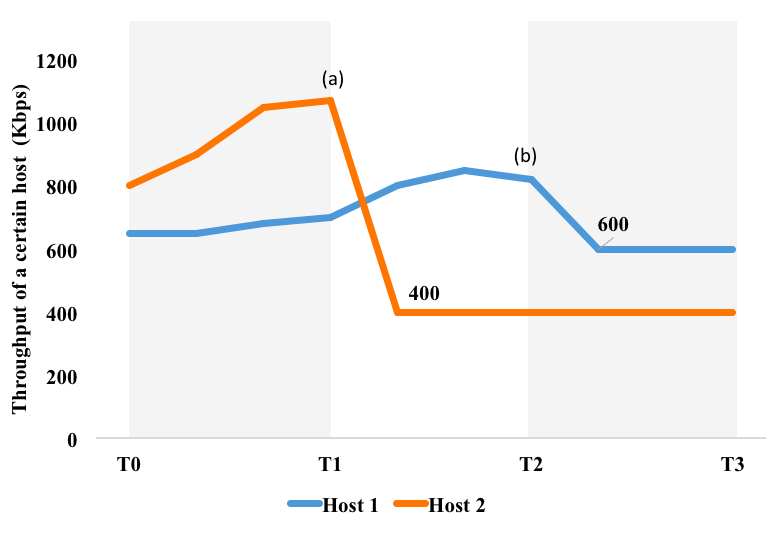
\includegraphics[width=3in]{./figures/mft_qos_rate_host}
\caption{Illustration of rate limiting for a certain host}
\label{fig:mft_qos_rate_host}
\end{figure}

\subsubsection{Rate Limitation of Applications}

An increasing number of network applications such as online games, video streaming, and conference calls are used. Therefore, substantial traffic exists in the network. Consequently, we integrated a flow classification engine to identify which application the flow belongs to. The integration scenario is presented in Fig. \ref{fig:class_classifying}.

To rate the limit for a certain application, we must first gather per-flow statistical information. When a connection is created, the first packet of the connection is handled by the forwarding service and the 5-tuple rules are added into the SDN switch to obtain the bandwidth information of the per-flow connection (see Section \ref{ssec:forwarding} for details). With the classified result of application identification, the application type of each connection can be determined.

When the network administrator requests to rate limit a certain application to a certain bandwidth, the bandwidth is equally distributed to each connection of the application. The controller sets all flows that belong to the same application into the same meter, and the bandwidth of the meter is modified to achieve the desired value. For example, suppose that we can determine which flows belong to an application through the flow classification engine. This application is to be limited to 1000 Kbps. In T0 (Fig. \ref{fig:mft_qos_rate_app}), three connections belong to this application, and the bandwidth of the meter to each link is set as 333 (1000/3) Kbps. In T2, two connections are added to this application, and the bandwidth of the meter to each link is reset as 200 (1000/5) Kbps. In T2, one connection is obtained in this application, and hence, the bandwidth of the meter to each link is reset as 250 (1000/4) Kbps. However, the sum of bandwidth from this application should always be 1000 Kbps. In other words, the bandwidth is dynamically adjusted.

It is worth noting that we did not change any rules in flow table; we merely change the bandwidth of the correspond meter in the meter table to reduce the overhead of switch and controller.

\begin{figure}[!t]
\centering
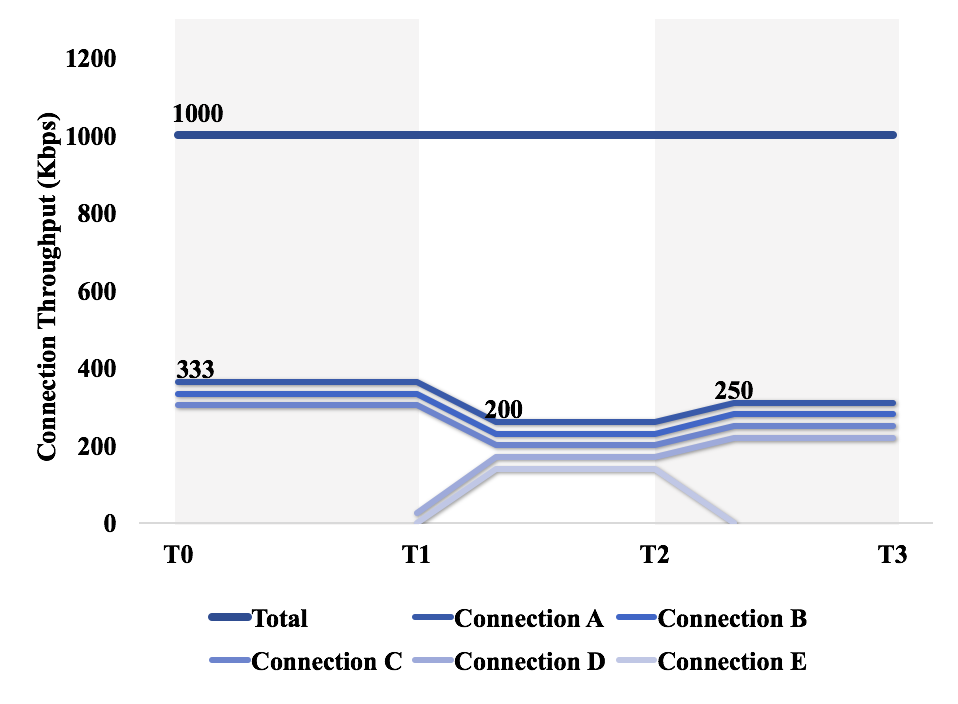
\includegraphics[width=3in]{./figures/mft_qos_rate_app}
\caption{Illustration of rate limiting for a certain application.}
\label{fig:mft_qos_rate_app}
\end{figure}

\subsubsection{The Flow Table Order of Forwarding and QoS Service}
Because the location of NAT, DHCP, and the firewall have been determined, we only need to decide the arrangement of QoS and forwarding. Assume that we place the QoS flow table after the forwarding flow table. In addition, we have only two services enabled, forwarding and QoS; therefore, the packet-in rule is in the last flow table of active service, Qos service. Then, suppose that a host is not limited by QoS policies. The first packet is not affected in both arrangements. For the subsequent packets, a difference can be observed. The packets that satisfy the rules in the forwarding flow table can not match rate limit rules in QoS flow table, because the host is not limited by QoS service; instead. As a result, the packets cause packet-in events by matching the packet-in rule in QoS service. This is unexpected because the packets already get the out-port action from the forwarding service. That is, it is not necessary to send these packet go to controller, and any packet-in event increases the controller’s load.

To reduce this load on the controller, we place the QoS flow table ahead of the forwarding flow table. In this scenario, all packets that pass through the QoS flow table continue to proceed to the forwarding flow table without satisfying any QoS rules. Then, all packets except the first packet are merely forwarded by the forwarding service instead of causing packet-in events. Thus, the controller’s load decreases.

\section{Performance Evaluation}
\subsection{Multiple Table Performance}

\begin{figure}[!t]
\centering
\includegraphics[width=3in]{./figures/evaluation_nat_scenario}
\caption{Multiple Table Performance Evaluation Scenario}
\label{fig:evaluation_nat_scenario}
\end{figure}

\begin{figure}[!t]
\centering
\includegraphics[width=3in]{./figures/evaluation_nat_result}
\caption{Results of Multiple Table Performance Evaluation}
\label{fig:evaluation_nat_result}
\end{figure}

Implementing a single flow table framework is easier than implementing a multiple flow table framework; however, multiple flow table frameworks are more flexible. To verify the efficiency of the multiple flow table vCPE framework, we conducted an experiment by using the NAT service to compare the throughput between single flow table vCPE and multiple flow table vCPE.

An overview of the experimental environment is presented in Fig. \ref{fig:evaluation_nat_scenario}. The NFV controller was run on the Dell PowerEdge R630 rack server, and the Pica8 P-3290 switch \cite{pica8-switch} was used as the SDN switch. We used iPerf2 \cite{iperf} to generate network traffic. The iPerf server connected the public IP address with 140.114.71.178, and then the iPerf client connected to the SDN switch and was controlled by the NFV controller. The NFV controller ran the NAT service, but used different frameworks, a single flow table and multiple flow table.

We used iPerf to generate UDP packets and send them to the server from the client, and we fixed the bandwidth at 100 Mbps. In this experiment, different payload sizes were used to evaluate the performance of the flow tables. As shown in Fig. \ref{fig:evaluation_nat_result}, the throughput values indicate that the performance for large packets such as 1024 bytes and 1470 bytes was higher than that for small packets.

Because the NAT service is required to set the packet header field and a small payload tends to result in more packets being sent to the server simultaneously, the performance for larger packets is high. The throughput value of the multiple table framework is close to that of the single table framework. Thus, the multiple table framework is more flexible than the single table framework; however, the performance of the frameworks is similar (Fig. \ref{fig:evaluation_nat_result}).

\subsection{Evaluation of QoS When Host Bandwidth Is Limited}

We verify our function by downloading a file, because downloading is a situation that always consumes network resources in practice. We downloaded an image of Ubuntu 14.04 that was approximately 1 GB in size.


The NFV controller ran on the Dell PowerEdge R630 rack server and executed QoS (Fig. \ref{fig:class_classifying}). The Edge-Core AS5712-54X \cite{edge-core-switch} switch was used as the OpenFlow-enabled switch with the PicOS TM r2.6 operating system.

We used a desktop computer as the experimental host to record the bandwidth every 2 s. As shown in Fig 13, we started downloading the file without rate limiting; the rate was between 190 000 and 410 000 Kbps initially. At the \nth{10} second, we limited the host bandwidth to 1024 Kbps and added the rule matching the destination MAC address with a meter of 1024 Kbps. Then, we determined that the bandwidth from this host decreased and was limited to approximately 1024 Kbps immediately.

At the \nth{36} second, we canceled the limit to this host. In other words, we removed the meter field from the rule in the flow table. We observed that the bandwidth of the download from this host rapidly increased without rate limiting.

\begin{figure}[!t]
\centering
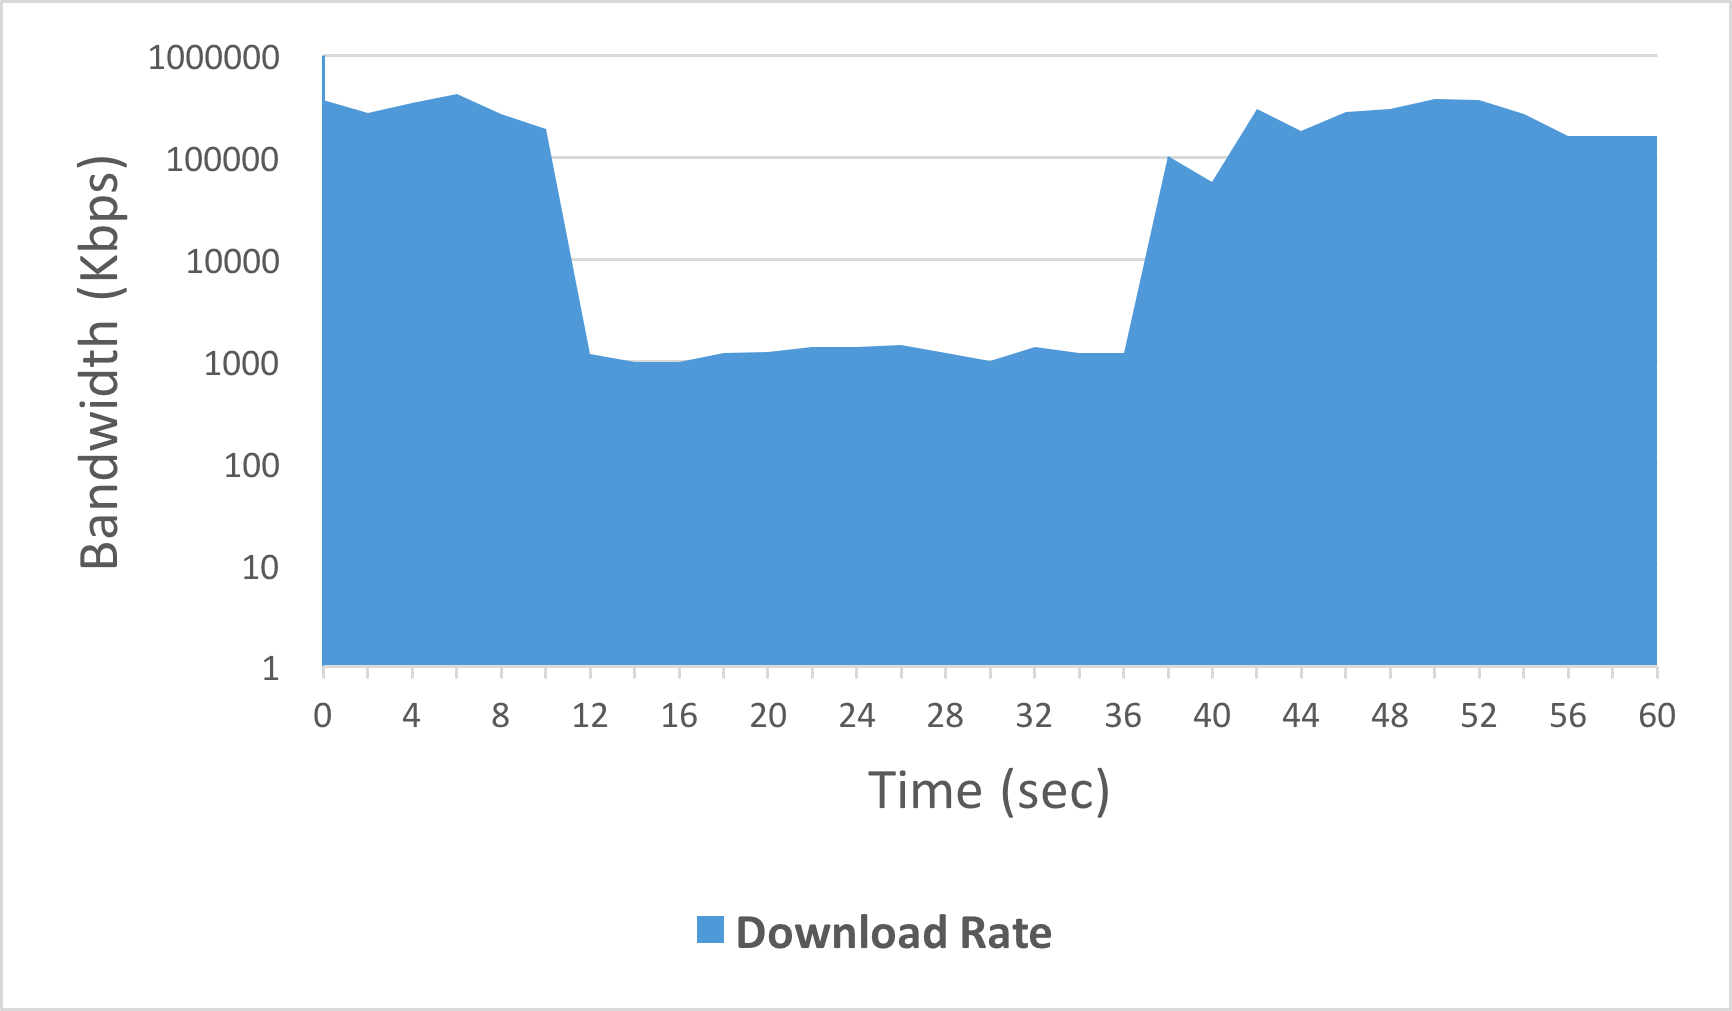
\includegraphics[width=3in]{./figures/qos_limit_host}
\caption{Limiting the download rate of a host.}
\label{fig:qos_limit_host}
\end{figure}

\begin{figure}[!t]
\centering
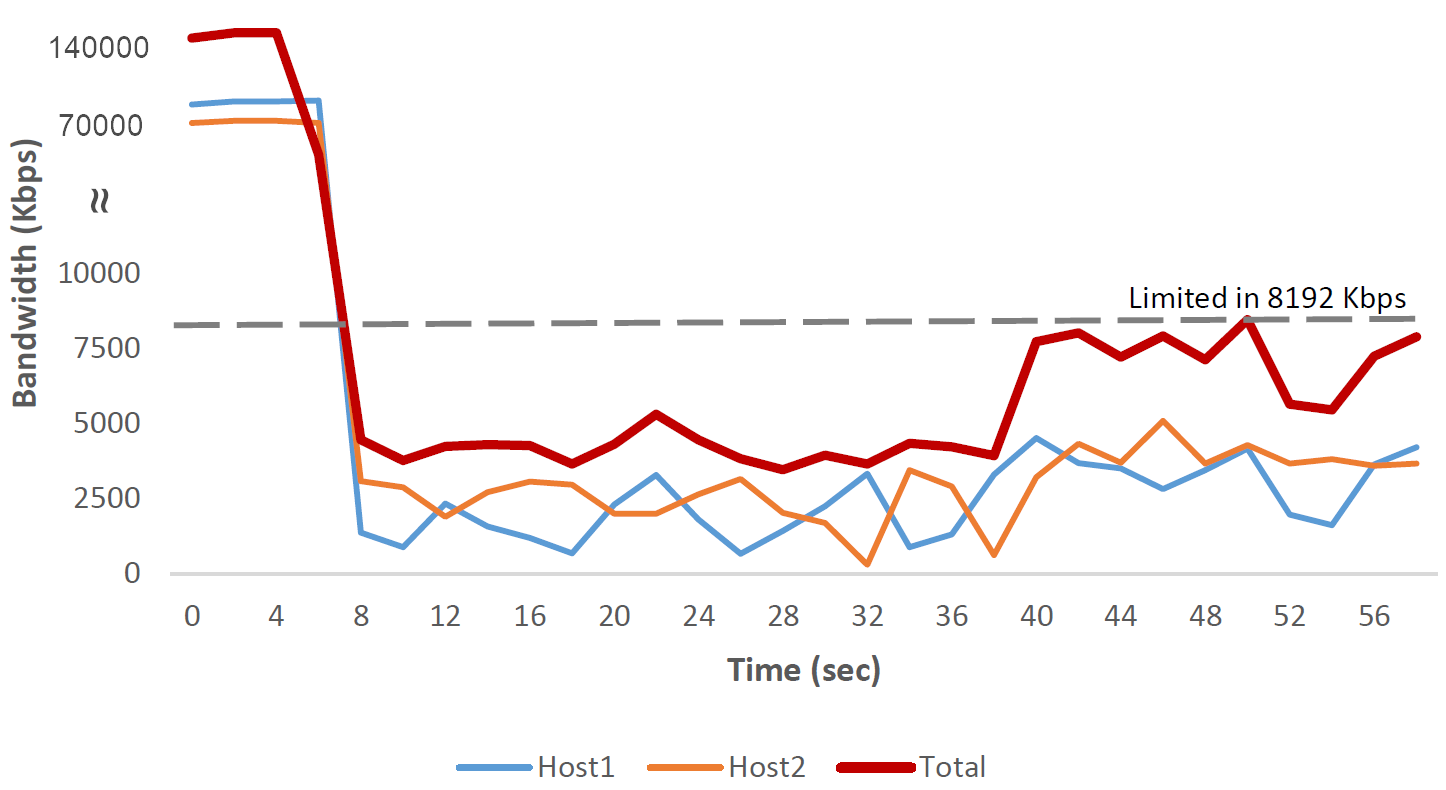
\includegraphics[width=3in]{./figures/mft_qos_rate_domain_app}
\caption{Limit the rate of Youtube in a network domain.}
\label{fig:mft_qos_rate_domain_app}
\end{figure}

\subsection{Evaluation of QoS When Application Bandwidth Is Limited}
Currently, numerous people use streaming applications, which consume a high amount of network resources. We employed application identification to determine the application to which each flow belongs.

In our experimental environment (Fig. \ref{fig:class_classifying}), we used a mirror switch to replicate all traffic from the SDN switch and to enable the application identification system to classify the flows according to the applications they belong to. The application identification system uploaded the identification results to the database.


Subsequently, the controller received the results from the database and updated the flow information of the applications. Therefore, we could use the flow information (5-tuple and identification results) to limit the application bandwidth.

We selected YouTube to verify our function for limiting applications and used three hosts (host 1, host 2, and host 3) in the same network domain. Then, we limited the bandwidth of YouTube in this network domain (i.e., the sum of bandwidths of host 1, host 2, and host 3).

Initially, without limitation, the total bandwidth of this network was approximately 3000 to 4000 Kbps (Fig. \ref{fig:mft_qos_rate_domain_app}). At the \nth{8} second, we limited the total bandwidth from YouTube to 2048 Kbps. We observed that the total traffic from YouTube in this network domain immediately decreased. Clearly, the total traffic from YouTube did not exceed the set bandwidth (2048 Kbps) because we limited YouTube in this network domain.

Using this function for limiting applications, we can guarantee that the traffic in a network domain does not exceed the network capacity, thus preventing traffic congestion.



\section{Conclusion and Future Works}
The proposed vCPE framework enables deploying NFVs as edge of network and these VNFs are implemented with multiple flow table management model. In this way, the customers only need a SDN switch at local network, and some network functions that could not be realized by single table mechanism are also resolved. The experimental results show that the framework provides better performance in VNF compete over single table SDN application. The integration evaluation also demonstrates its flexibility to integrate with any other bonus application identification system, IDS or IPS

This paper implemented multiple VNF cascade system over the single-table sdn switch. However, the multi-table environment in experiment basing on the single-table switch environment can't achieve the better performance compare with single-table switch. Although the multi-table based sdn switches are available on the market, those switches have different supporting table for different flow entry which might not be compatible to the customer requirement .If the algorithm is not appropriate designed for the specific network application entry, it will cause system crashed. We plan to design the algorithms specifically for multi-table switch in order to minimize the possibility of the crash of the system and maximize the performance.

\bibliographystyle{ieeetr}
\bibliography{paper}



\end{document}
